\documentclass[11pt]{article}

\usepackage[utf8]{inputenc}
\usepackage[T1]{fontenc}
\usepackage[spanish,es-nodecimaldot]{babel}
\usepackage{mathptmx}
\usepackage[margin=2.3cm]{geometry}
\usepackage{microtype}
\usepackage{amsmath}
\usepackage{graphicx}
\graphicspath{{figuras/}}
\usepackage{enumitem}
\usepackage{titlesec}
\usepackage{parskip}

\titleformat{\section}{\normalfont\bfseries\large}{}{0pt}{}
\titlespacing*{\section}{0pt}{12pt}{4pt}
\titleformat{\subsection}{\normalfont\bfseries}{}{0pt}{}
\titlespacing*{\subsection}{0pt}{8pt}{2pt}
\setlist[itemize]{leftmargin=1.2em,itemsep=2pt,topsep=2pt}
\setlist[enumerate]{leftmargin=1.6em,itemsep=3pt,topsep=3pt}
\pagestyle{empty}
\setlength{\parskip}{5pt}
\hyphenpenalty=10000
\exhyphenpenalty=10000
\emergencystretch=2em

\begin{document}

\begin{center}
	{\small SMAII, Redes Complejas Multicapa}\\[6pt]
	{\Large\bfseries Proyecto final: sección de Metodología}\\[3pt]
	{\normalsize Efecto de una campaña sobre la opinión colectiva y predicción de su conveniencia}\\[4pt]
	{\small Octubre de 2026}
\end{center}

\section*{Integrantes del equipo}
\begin{itemize}
	\item Jorge Miyoshi Mikami Alonso
	\item Luis Manuel Reyes Colín
\end{itemize}

\section*{Metodología}

Todo el proyecto se hizo con simulaciones por computadora; no usamos encuestas ni datos reales.
Creamos poblaciones artificiales de personas, les dimos reglas sencillas para conversar entre ellas
y con la campaña, y observamos cómo terminaban sus opiniones y su conducta. Las reglas de opinión
salen de Pansanella \emph{et al.} \cite{Pansanella2023} y las de conducta de Yin \emph{et al.}
\cite{Yin2025}.

Programamos todo en Python. Las redes se construyeron con NetworkX \cite{Hagberg2008}, las
simulaciones se escribieron con NumPy (y Numba para que corrieran más rápido), los resultados se
guardaron en tablas de pandas y el aprendizaje automático se hizo con scikit-learn
\cite{Pedregosa2011}. Cada simulación usa una semilla aleatoria guardada, así que se puede repetir
exactamente igual. La Figura~\ref{fig:flujo} resume el orden del trabajo; abajo explicamos cada paso
siguiendo los objetivos particulares.

\begin{figure}[h]
	\centering
	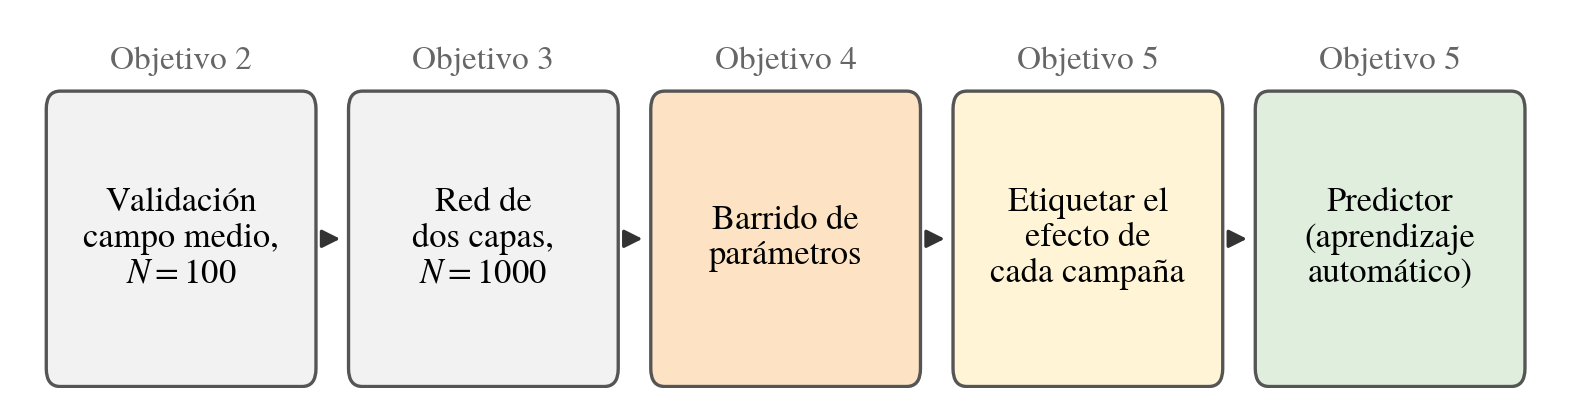
\includegraphics[width=\textwidth]{flujo_trabajo}
	\caption{Orden en que se desarrolló el trabajo y objetivo particular al que corresponde cada etapa.}
	\label{fig:flujo}
\end{figure}

\subsection*{1. Búsqueda bibliográfica}

Empezamos por los dos artículos de referencia y revisamos los trabajos que citan y los que los citan
a ellos. Así llegamos al modelo original de Deffuant \emph{et al.} \cite{Deffuant2000} y al de sesgo
algorítmico de Sîrbu \emph{et al.} \cite{Sirbu2019}. También buscamos en Google Scholar y Scopus
con palabras como \emph{bounded confidence}, \emph{algorithmic bias}, \emph{mass media} y
\emph{multiplex opinion dynamics}. Con esto escribimos los antecedentes y elegimos las reglas y los
valores que usamos después.

\subsection*{2. Modelo de opinión y su validación}

Cada persona $i$ tiene una opinión $x_i$, un número entre 0 y 1, donde 0 y 1 son las posturas más
extremas. La simulación avanza repitiendo una misma interacción (Figura~\ref{fig:paso}):

\begin{enumerate}
	\item Se escoge a una persona $i$ al azar.

	\item La plataforma le muestra a uno de sus contactos $j$. No lo escoge al azar: entre más
	      parecida sea la opinión de $j$ a la de $i$, más probable es que se lo muestre. Qué tanto
	      favorece a los parecidos lo controla el sesgo algorítmico $\gamma$ (con $\gamma=0$ todos los
	      contactos tienen la misma probabilidad).

	\item Si sus opiniones están a menos de $\epsilon$ de distancia, ambos cambian su opinión al
	      promedio de las dos. Si están más lejos, no pasa nada.

	\item Con probabilidad $p_m$, la persona $i$ además ve la campaña, que siempre dice lo mismo
	      ($x_m$). Si la campaña está dentro de su umbral, $i$ se mueve al promedio entre su opinión y
	      $x_m$. La campaña nunca cambia.
\end{enumerate}

Llamamos \emph{paso} a $N$ repeticiones de lo anterior, de modo que en promedio cada persona tiene
una interacción por paso.

Antes de agregar la red y la segunda capa, comprobamos que el programa funcionaba bien
reproduciendo el caso más simple de Pansanella \emph{et al.}: 100 personas donde todos pueden hablar
con todos, opiniones iniciales repartidas al azar entre 0 y 1, y sus mismos valores de $\epsilon$,
$\gamma$ y $p_m$, con 100 repeticiones de cada combinación. Corrimos sus cuatro escenarios: una
campaña moderada ($x_m=0.5$), una extremista ($x_m=0$), dos medios opuestos ($0.05$ y $0.95$) y esos
dos más uno moderado. Dimos por bueno el programa si el número promedio de grupos de opinión y el
porcentaje de personas alrededor del medio se parecían a sus gráficas. Estas corridas quedaron
guardadas como pruebas automáticas del código.

\begin{figure}[h]
	\centering
	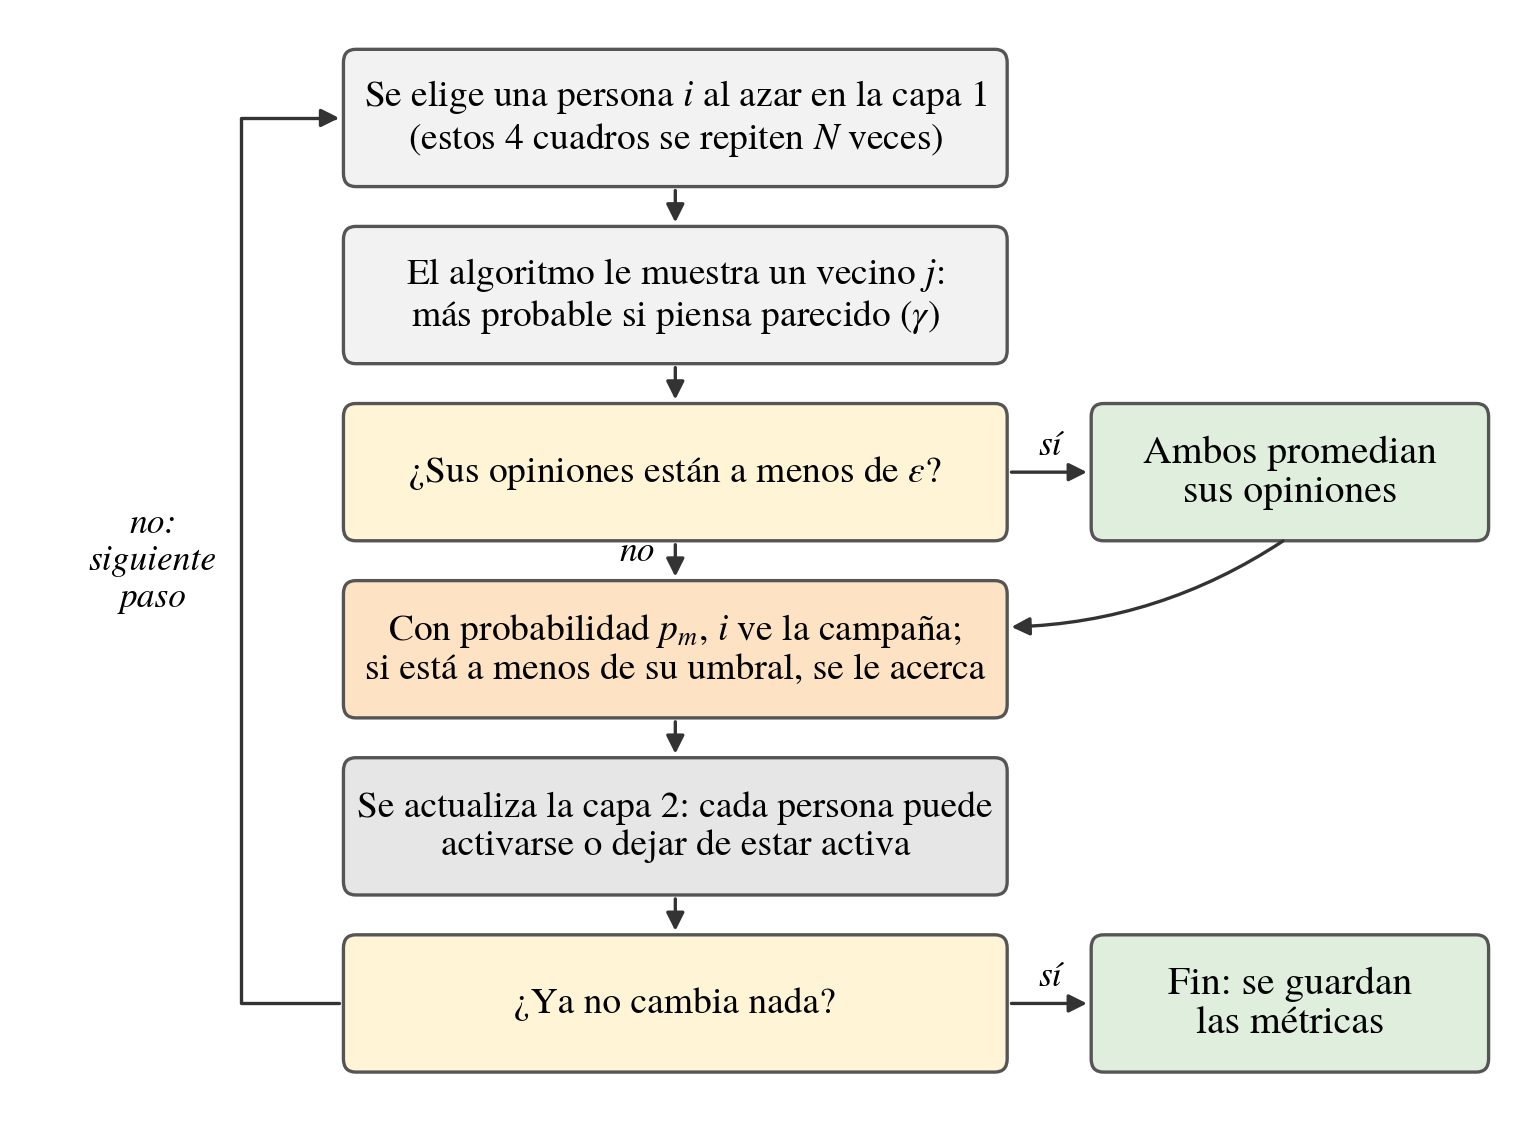
\includegraphics[width=0.88\textwidth]{paso_simulacion}
	\caption{Lo que ocurre en un paso de la simulación.}
	\label{fig:paso}
\end{figure}

\subsection*{3. Construcción de la red de dos capas}

Simulamos una población de $N=1000$ personas que viven al mismo tiempo en dos redes, una para lo que
opinan y otra para lo que hacen (Figura~\ref{fig:red}). En las dos capas los \textbf{nodos} son las
mismas personas. Lo único que conecta las capas es que cada persona está en ambas: lo que le pasa
en una capa cambia sus reglas en la otra. No usamos símplices; todas las interacciones son entre dos
personas.

\begin{figure}[h]
	\centering
	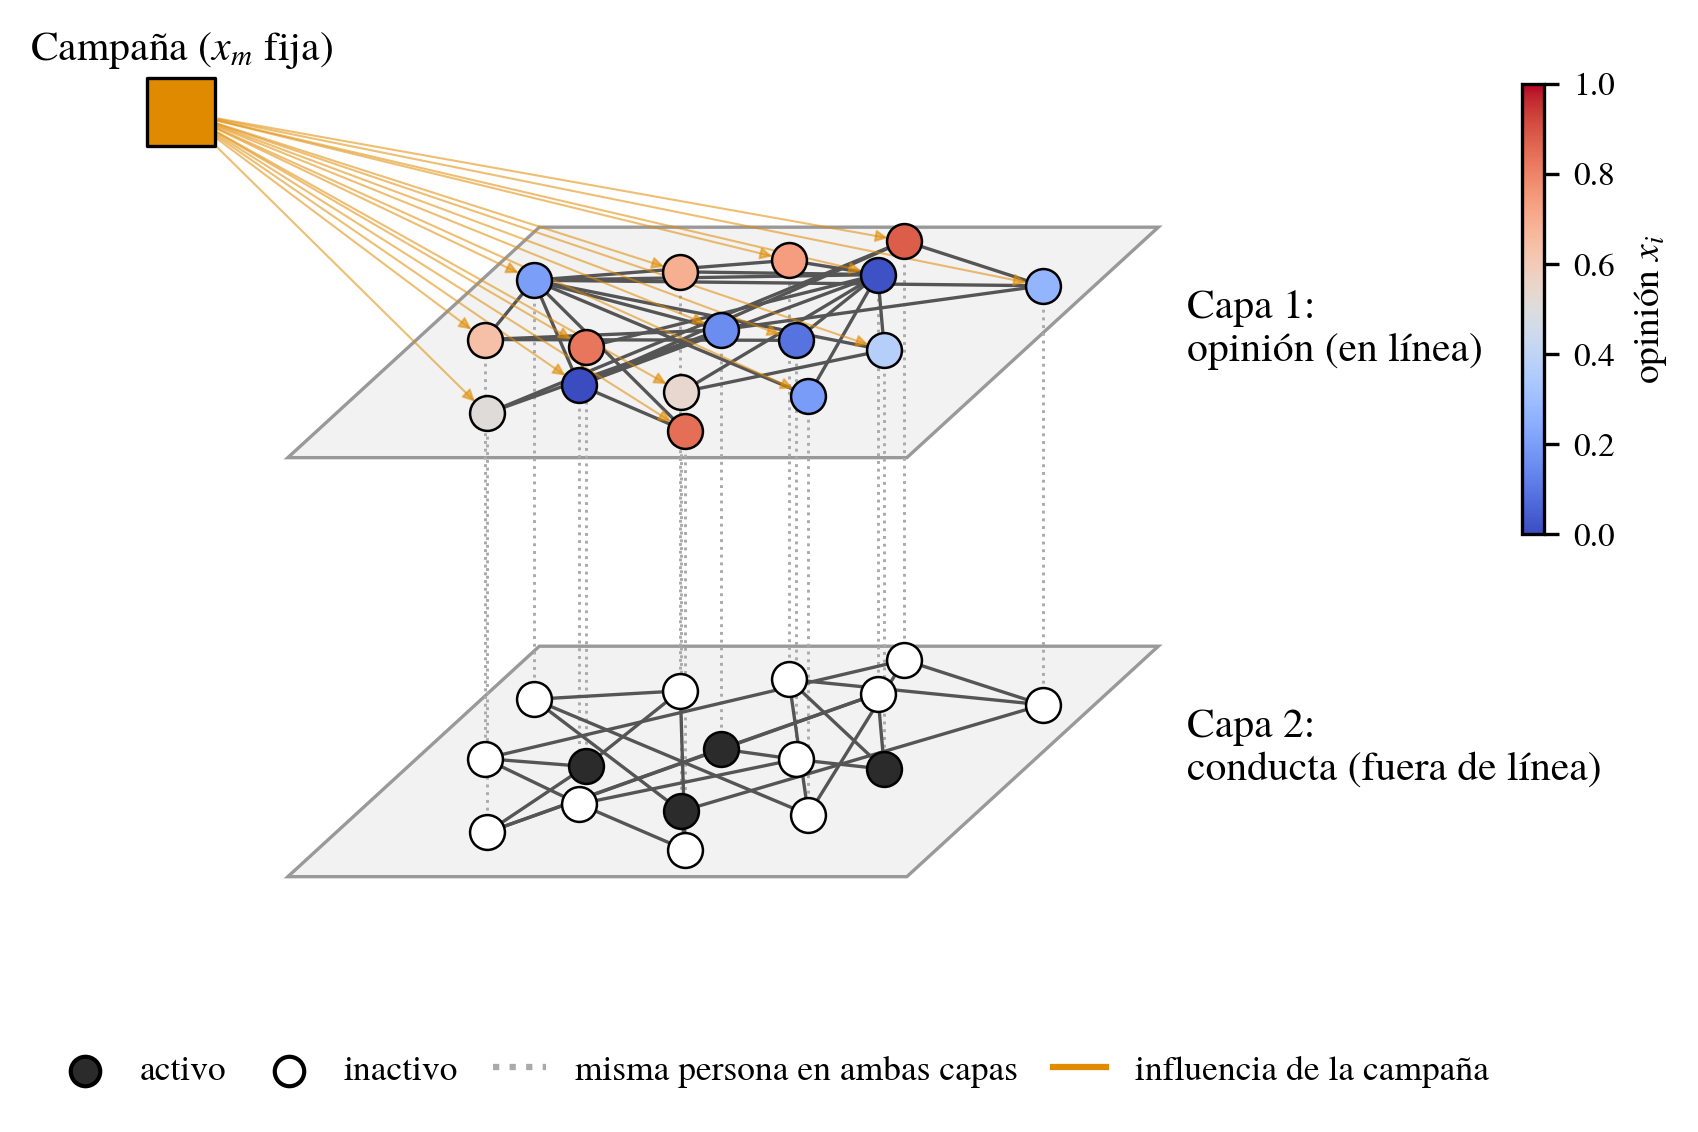
\includegraphics[width=0.92\textwidth]{red_dos_capas}
	\caption{Esquema de la red (con pocos nodos, solo para ilustrar). Arriba, cada color es una opinión;
	abajo, negro es activo y blanco inactivo. La línea punteada une a la misma persona en las dos capas
	y las flechas naranjas salen de la campaña hacia todos.}
	\label{fig:red}
\end{figure}

\textbf{Capa 1, opinión (en línea).} Una arista entre dos personas quiere decir que se siguen en una
red social y pueden ver lo que publica la otra. Las aristas son \textbf{no dirigidas}, porque la
influencia va en ambos sentidos, y \textbf{no tienen peso fijo}. Lo que sí cambia con el tiempo es la
probabilidad de que una arista se use: el sesgo algorítmico hace que se usen más las que unen
opiniones parecidas, así que esa probabilidad funciona como un peso que cambia según las opiniones.
Probamos dos formas de red, ambas con 8 contactos por persona en promedio: una Erd\H{o}s--Rényi
\cite{Erdos1959}, donde los contactos se reparten al azar y todos tienen más o menos los mismos, y
una Barabási--Albert \cite{Barabasi1999}, donde unos pocos tienen muchísimos contactos, como pasa en
las redes sociales reales.

\textbf{La campaña.} La campaña es un nodo extra que no forma parte de ninguna capa. Tiene una arista
\textbf{dirigida} hacia cada persona de la capa 1: ella influye en todos, pero nadie influye en ella.
Estas aristas tampoco tienen peso; qué tan seguido se ve la campaña lo decide $p_m$. En el
experimento principal hay una sola campaña; los casos con dos o tres medios solo se usaron para
validar.

\textbf{Capa 2, conducta (fuera de línea).} Aquí cada persona solo puede estar \emph{activa} o
\emph{inactiva}, lo que representa la conducta que busca la campaña: comprar, votar o asistir. Una
arista representa contacto en persona (familia, trabajo, vecinos); es no dirigida y sin peso. Como en
Yin \emph{et al.}, todos tienen 4 contactos en esta capa, elegidos al azar e independientes de la
capa 1: tus amigos en redes no son los mismos que ves en persona.

Para describir cada capa calculamos medidas estructurales básicas: grado promedio y distribución de
grado, coeficiente de agrupamiento, longitud promedio de caminos, cuántas aristas comparten ambas capas
y qué tanto se agrupan las personas de opinión parecida al final.

\subsection*{Cómo se influyen las dos capas}

\textbf{De la opinión a la conducta.} Entre más cerca esté una persona de lo que dice la campaña, más
fácil se activa y menos probable es que lo deje. Una persona inactiva puede contagiarse de cada
vecino activo, y una activa puede dejar de serlo, igual que en un modelo epidémico tipo SIS. Usamos
las probabilidades de Yin \emph{et al.}, ajustadas según la cercanía de cada persona a la campaña,
$1-|x_i-x_m|$. Al inicio, el $10\%$ de las personas, elegidas al azar, está activo.

\textbf{De la conducta a la opinión.} En Yin \emph{et al.} consumir más hace que sea más fácil volverse
optimista. Nosotros lo trasladamos así: entre más contactos activos tenga una persona en la capa 2,
más abierta está a escuchar a la campaña. Su umbral frente a la campaña crece según
\[
\epsilon_i^{m}=\epsilon\,(1+\alpha f_i),
\]
donde $f_i$ es la fracción de sus contactos de la capa 2 que están activos y $\alpha$ mide qué tan
fuerte es este efecto (si $\alpha=0$, la conducta no afecta la opinión). Con otras personas sigue
usando su umbral normal $\epsilon$.

En cada paso se actualiza primero la capa 1 y después la capa 2. La simulación termina cuando ya no
cambia nada (durante 100 pasos seguidos ninguna opinión se mueve más de $10^{-4}$ y casi nadie se
activa ni se desactiva) o al llegar a $10^4$ pasos, porque con una campaña presente a veces el sistema
nunca se queda quieto.

\subsection*{4. Barrido de parámetros y métricas del estado final}

Corrimos la simulación para todas las combinaciones del Cuadro~\ref{tab:barrido}. Basta con
campañas de $x_m=0$ a $0.5$ porque el caso del otro lado es simétrico. Para que el predictor
aprendiera a reconocer distintas poblaciones, las opiniones iniciales no siempre se repartieron
parejo: usamos cuatro casos, una población uniforme, una concentrada en el centro, una dividida en
los dos extremos y una cargada hacia el lado contrario de la campaña. Cada combinación se repitió
10 veces. Las corridas con $p_m=0$ son la misma población sin campaña, así que nos sirvieron para
comparar ``con campaña'' contra ``sin campaña''.

\begin{table}[h]
	\centering
	\small
	\begin{tabular}{lll}
		\hline
		Parámetro & Qué representa & Valores \\
		\hline
		$\epsilon$ & qué tan abierta es la población & $0.1, 0.2, 0.3, 0.4, 0.5$ \\
		$\gamma$ & sesgo del algoritmo & $0, 0.5, 0.75, 1, 1.25, 1.5$ \\
		$p_m$ & qué tan seguido se ve la campaña & $0, 0.1, 0.2, 0.3, 0.4, 0.5$ \\
		$x_m$ & qué postura promueve la campaña & $0, 0.1, 0.2, 0.3, 0.4, 0.5$ \\
		$\alpha$ & efecto de la conducta en la opinión & $0, 0.5, 1$ \\
		capa 1 & forma de la red de opinión & Erd\H{o}s--Rényi, Barabási--Albert \\
		$x_i(0)$ & opiniones iniciales & 4 casos \\
		\hline
		fijos & personas, contactos en capa 1 y 2 & $N=1000$, $8$, $4$ \\
		\hline
	\end{tabular}
	\caption{Valores usados en el barrido de parámetros.}
	\label{tab:barrido}
\end{table}

Al final de cada corrida medimos: cuántos grupos de opinión quedaron, qué tan parejos son de tamaño,
qué porcentaje de personas quedó junto a la campaña, qué tan polarizada quedó la población, qué
tanto se acercaron en promedio a la campaña, qué fracción quedó activa y cuánto tardó en
estabilizarse. Su definición está en el Marco Teórico.

\subsection*{5. Clasificación de los estados finales y predictor}

Primero describimos cada resultado como consenso (casi todos en un grupo), polarización (dos grupos
grandes) o fragmentación (muchos grupos). Después comparamos cada corrida con su versión sin campaña
y le pusimos una etiqueta:

\begin{itemize}
	\item \textbf{Favorable:} la campaña juntó a más de $5\%$ más de personas cerca de su postura, sin
	      hacer crecer al grupo que quedó fuera de su alcance.
	\item \textbf{Contraproducente:} el grupo fuera de su alcance creció más de $5\%$, o la fracción de
	      activos bajó más de $5\%$.
	\item \textbf{Neutra:} cualquier otro caso.
\end{itemize}

Luego entrenamos un modelo que adivina esa etiqueta usando solo lo que se sabe \emph{antes} de lanzar
la campaña: los parámetros del Cuadro~\ref{tab:barrido} y algunos datos de la población inicial (su
opinión promedio, qué tan dispersa está, si está dividida en dos y cuántas personas están desde el
inicio a menos de $\epsilon$ de la campaña). Probamos tres modelos de scikit-learn: regresión
logística, bosque aleatorio y \emph{gradient boosting}. Para revisar que el modelo funcionara con
casos nuevos, apartamos el $20\%$ de las combinaciones de parámetros y solo las usamos al final para
evaluarlo. Medimos qué tanto acierta (exactitud, F1 y matriz de confusión) y qué variables pesan más.
Como queríamos una regla fácil de usar, también entrenamos un árbol de decisión pequeño (máximo 4
preguntas), que se puede leer como una lista de condiciones.

\subsection*{6. Análisis y comparación}

Presentamos los resultados con mapas de calor como los de Pansanella \emph{et al.}, para comparar
directamente, y con gráficas de la fracción de activos contra $\alpha$ para buscar los saltos bruscos
que reporta Yin \emph{et al.} Con eso revisamos si sus conclusiones siguen valiendo cuando hay red y
conducta: si una población abierta sigue siendo más fácil de manipular, si repetir de más un mensaje
moderado sigue creando minorías extremistas y si el sesgo algorítmico sigue frenando la
radicalización. Por último, vimos en qué casos se equivoca más el predictor.

\begin{thebibliography}{9}
\setlength{\itemsep}{3pt}

\bibitem{Deffuant2000}
G. Deffuant, D. Neau, F. Amblard and G. Weisbuch, \emph{Mixing beliefs among interacting agents}, Advances in Complex Systems \textbf{3} (2000) 87--98.

\bibitem{Pansanella2023}
V. Pansanella, A. Sîrbu, J. Kertesz and G. Rossetti, \emph{Mass media impact on opinion evolution in biased digital environments: a bounded confidence model}, Scientific Reports \textbf{13} (2023) 14600.

\bibitem{Yin2025}
L. Yin, J. Chen, F. Gao and X. Wu, \emph{Coevolution of opinion and consumption behavior under a two-layer network framework}, Physica A \textbf{680} (2025) 131020.

\bibitem{Sirbu2019}
A. Sîrbu, D. Pedreschi, F. Giannotti and J. Kertész, \emph{Algorithmic bias amplifies opinion fragmentation and polarization: a bounded confidence model}, PLoS ONE \textbf{14} (2019) e0213246.

\bibitem{Erdos1959}
P. Erd\H{o}s and A. Rényi, \emph{On random graphs I}, Publicationes Mathematicae Debrecen \textbf{6} (1959) 290--297.

\bibitem{Barabasi1999}
A.-L. Barabási and R. Albert, \emph{Emergence of scaling in random networks}, Science \textbf{286} (1999) 509--512.

\bibitem{Hagberg2008}
A. Hagberg, D. Schult and P. Swart, \emph{Exploring network structure, dynamics, and function using NetworkX}, Proceedings of the 7th Python in Science Conference (2008) 11--15.

\bibitem{Pedregosa2011}
F. Pedregosa \emph{et al.}, \emph{Scikit-learn: machine learning in Python}, Journal of Machine Learning Research \textbf{12} (2011) 2825--2830.

\end{thebibliography}

\end{document}
